\documentclass[12pt,a4paper]{article}

% To use this template make changes to following:
% 1. Fill-ables section.
% 2. Instructions.
% 3. Marks table.
% 4. Actual questions.

% ================================ 1. Fill-ables ================================
\newcommand\University{National University of Computer and Emerging Sciences}
\newcommand\Department{School of Engineering}
\newcommand\Campus{Islamabad Campus}
\newcommand\Semester{Spring 2015}
\newcommand\Exam{Sessional--I}
\newcommand\Subject{CS210--Data Structures and Algorithms}
\newcommand\ExamDate{Monday, March 16, 2015}
\newcommand\InstructorOne{Attique Dawood}
\newcommand\InstructorTwo{\null~}
\newcommand\InstructorThree{\null}
\newcommand\TotalTime{01 Hours}
\newcommand\TotalMarks{50}
\newcommand\TotalQuestions{5}
\newcommand\TotalPages{\pageref{LastPage}} % Automatic: No need to change this.
% Marks of each question
\def\Qone{10}
\def\Qtwo{10}
\def\Qthree{10}
\def\Qfour{10}
\def\Qfive{10}
\def\Qsix{0}
\def\Qseven{0}
\def\Qeight{0}
\def\Qnine{0}
\def\Qten{0}
% ============================================================================

% ============== 2. Packages ==============
\usepackage{amsmath}
\usepackage{float}
\usepackage{graphicx}
\usepackage[hyphens]{url}
\usepackage[hidelinks]{hyperref}	% Clickable links to figures, references and urls.
\usepackage{lastpage}
\usepackage{array}
\usepackage{fancyhdr}
% Drawing packages.
\usepackage{pgf}
\usepackage{tikz}
% Listings for formatting code.
\usepackage{listings}
\usepackage{textcomp}

% General listings options.
\lstset{breaklines=true, basicstyle=\footnotesize\ttfamily, tabsize=4, numbers=left, stepnumber=1, frame=none, showstringspaces=false, upquote=true}
% C++ specific high-lighting. Comments are 50/50 shades of green/black and strings coloured with 60/40 red/black mixture.
\lstset{language=[ISO]C++, commentstyle=\color{green!50!black}, keywordstyle=\color{blue}, stringstyle=\color{red!60!black}}

% Table cell alignment directives.
\newcolumntype{L}[1]{>{\raggedright\let\newline\\\arraybackslash\hspace{0pt}}m{#1}}
\newcolumntype{C}[1]{>{\centering\let\newline\\\arraybackslash\hspace{0pt}}m{#1}}
\newcolumntype{R}[1]{>{\raggedleft\let\newline\\\arraybackslash\hspace{0pt}}m{#1}}

% Line spacing.
\def\SingleSpacing{\def\baselinestretch{1}\large\normalsize}
\def\DoubleSpacing{\def\baselinestretch{1.5}\large\normalsize}

% Margins.
\setlength{\oddsidemargin}{0in}
\setlength{\evensidemargin}{0in}
\setlength{\headheight}{28pt}
\setlength{\headsep}{2.5pt}
\setlength{\topmargin}{-55pt}
\setlength{\textwidth}{6.5in}
\setlength{\textheight}{10.75in} % Actual: 10.75in

% ============================= 3. Header and Footer ============================
\pagestyle{empty}
% Header
\chead
{
	{\large\textbf{\University}}\\
	\begin{minipage}{0.45\textwidth}
	\begin{center}
	{\small\textbf{\Department}}
	\end{center}
	\end{minipage}
	\begin{minipage}{0.45\textwidth}
	\begin{center}
	{\small\textbf{\Campus}}
	\end{center}
	\end{minipage}
}
% Footer
\lfoot{{\small\Exam}}
\cfoot{{\small\Semester}}
\rfoot{{\small Page \textbf{\thepage}~of \textbf{\TotalPages}}}
\renewcommand{\headrulewidth}{0.4pt}
\renewcommand{\footrulewidth}{0.4pt}
% ================================= 4. Front Page ===============================
\begin{document}
% A cute macro to add up marks of all individual questions. Uncomment if you want to use this.
\pgfmathtruncatemacro\TotalMarks{\Qone+\Qtwo+\Qthree+\Qfour+\Qfive+\Qsix+\Qseven+\Qeight+\Qnine+\Qten}
% Use this macro if marks are in decimal points
%\newcommand\TotalMarks{\pgfmathsetmacro\TotalMarks{\Qone+\Qtwo+\Qthree+\Qfour+\Qfive+\Qsix+\Qseven+\Qeight+\Qnine+\Qten}}
\begin{minipage}[t]{0.6\textwidth}
\begin{flushleft}
\DoubleSpacing
{\Large\textbf{\Subject}}\\
{\normalsize\ExamDate}\\
{\large\textbf{Course Instructor}}\\
{\normalsize\InstructorOne}\\
{\normalsize\InstructorTwo}\\
{\normalsize\InstructorThree}
\end{flushleft}
\end{minipage}
\begin{minipage}[t]{0.01\textwidth}
~
\end{minipage}
\begin{minipage}[t]{0.325\textwidth}
\DoubleSpacing
{\normalsize Serial No:}\\
{\Large\textbf{\Exam}}\\
{\large\textbf{Total Time: \TotalTime}}\\
{\large\textbf{Total Marks: \TotalMarks}}\\[1cm]
\rule{5cm}{0.2mm}\\[-0.25cm]
{\small Signature of Invigilator}
\end{minipage}
\SingleSpacing
~\\[1.5cm] % Extra space.
\rule{7cm}{0.2mm}~\rule{2.5cm}{0.2mm}~\rule{2cm}{0.2mm}~\rule{4.5cm}{0.2mm}\\
{\small Student Name\hspace{4.75cm}Roll No\hspace{1.35cm}Section\hspace{0.95cm}Signature}\\[1cm]
% ============================ 5. Instructions ==================================
\textbf{DO NOT OPEN THE QUESTION BOOK OR START UNTIL INSTRUCTED.}\\
\textbf{Instructions:}
\begin{enumerate}
\itemsep0em
\item Verify at the start of the exam that you have a total of \TotalQuestions~questions printed on \TotalPages~pages including this title page.
\item Attempt all questions on the question-book and in the given order.
\item The exam is closed books, closed notes. Please see that the area in your threshold is free of any material classified as `useful in the paper' or else there may be a charge of cheating.
\item Read the questions carefully for clarity of context and understanding of meaning and make assumptions wherever required, for neither the invigilator will address your queries, nor the teacher/examiner will come to the examination hall for any assistance.
\item Fit in all your answers in the provided space. You may use extra space on the last page if required. If you do so, clearly mark question/part number on that page to avoid confusion. 
\item Use only your own stationery and calculator. If you do not have your own calculator, use manual calculations. 
\item Use only permanent ink-pens. Only the questions attempted with permanent ink-pens will be considered. Any part of paper done in lead pencil cannot be claimed for checking/rechecking.
\item \textbf{All distances and dimensions are in meters}.
\end{enumerate}
% =============================== 6. Marks Table ================================
\begin{table}[H]
\begin{center}
\vspace{0.3cm}
	{\footnotesize \begin{tabular}{|C{1.8cm}|C{0.75cm}|C{0.75cm}|C{0.75cm}|C{0.75cm}|C{0.75cm}|c|}
	\hline
		\rule{0pt}{4.6ex} & Q-1 & Q-2 & Q-3 & Q-4 & Q-5 &\textbf{Total}\\[-0.5ex]
		\hline
		\rule{0pt}{2.5ex}\textbf{Total Marks}& \Qone & \Qtwo & \Qthree & \Qfour & \Qfive & \TotalMarks\\
		\hline
		\rule{0pt}{2.5ex}\textbf{Marks Obtained}& & & & & &\\
	\hline
	\end{tabular}}
\end{center}
\end{table}
{\small \textbf{Vetted By: \rule{6cm}{0.2mm} Vetter Signature: \rule{4.5cm}{0.2mm}}}
\setlength{\textheight}{10.4in}
\newpage
\pagestyle{fancy}
% ================================== 7. Questions ===============================
\noindent\textbf{Question 1: Complexity Analysis \hfill \Qone~marks}
\begin{itemize}
\item[a.] Arrange the following in increasing order of complexity: $\log n$, $n logn$, $n^2$, $n!$, $n\log n$, $n$, $n^2\log n$, $e^n$.\vspace{8cm}
\item[b.] Find the Big O of following code segment:
\begin{lstlisting}
// Input is n
int i=1;
while (true)
{
	if (i>n*n)
		break;
	for (int j=10; j<n; j++)
	{
		// Do nothing.
	}
	i=i*3;
}
\end{lstlisting}
\end{itemize}
\newpage
\noindent\textbf{Question 2: Linked List and Priority Queues\hfill \Qtwo~marks}
\begin{itemize}
\item[a.] With the help of figure(s) illustrate the sequence of operations to delete a node in doubly--linked list. Don't write code.\vspace{8cm}
\item[b.] Following sequence of data with given priorities is inserted in a priority queue. Show priority queue after each insertion\\
\begin{table}[H]
\begin{center}
\vspace{0.3cm}
\SingleSpacing
	\begin{tabular}{lcccccc}
	\hline \hline
		\rule{0pt}{2.6ex}Sequence & 1 & 2& 3& 4& 5& 6\\
		\hline
		\rule{0pt}{2.6ex}Data & A & B& C& D& E& F\\
		Priority& 10 & 5& 12& 2& 18& 11\\
	\hline \hline
	\end{tabular}
\end{center}
\end{table}
\end{itemize}

\newpage
\noindent\textbf{Question 3: Ordered Tree\hfill \Qthree~marks}\\[0.2cm]
\begin{tikzpicture} [level/.style={sibling distance=60mm/#1}]
\node[circle,draw] (r){$R$}
child
{
	node[circle,draw] (1){$1$}
	child{node[circle,draw] (4){$4$}}
	child
	{
		node[circle,draw] (5){$5$}
		child{node[circle,draw] (10){$10$}}
		child{node[circle,draw] (11){$11$}}
	}
}
child
{
	node[circle,draw] (2){$2$}
	child{node[circle,draw] (6){$6$}}
	child
	{
		node[circle,draw] (7){$7$}
		child{node[circle,draw] (12){$12$}}
		child{node[circle,draw] (13){$13$}}
	}
	child{node[circle,draw] (8){$8$}}
}
child
{
	node[circle,draw] (3){$3$}
	child
	{
		node[circle,draw] (9){$9$}
		child{node[circle,draw] (14){$14$}}
		child{node[circle,draw] (15){$15$}}
	}
};
\end{tikzpicture}\\[0.2cm]
Answer the following questions related to given tree.
\begin{itemize}
\item[a.] What is the preorder number of 11 in tree?
\item[b.] What is the height of 1?
\item[c.] What is the depth of 7?
\item[d.] What is the right child of 5?
\item[e.] Find expressions for following traversals: \verb|Preorder(1)|, \verb|Inorder(2)| and \verb|Postorder(R)|.
\end{itemize}
%\begin{tikzpicture} [level/.style={sibling distance=60mm/#1}]
%\node[circle,draw] (r){$\times$}
%child
%{
%	node[circle,draw] (1){$-$}
%	child{node[circle,draw] (4){$a$}}
%	child
%	{
%		node[circle,draw] (5){$\times$}
%		child{node[circle,draw] (10){$b$}}
%		child{node[circle,draw] (11){$c$}}
%	}
%}
%child
%{
%	node[circle,draw] (2){$+$}
%	child
%	{
%		node[circle,draw] (7){$\div$}
%		child{node[circle,draw] (12){$d$}}
%		child{node[circle,draw] (13){$e$}}
%	}
%	child{node[circle,draw] (8){$f$}}
%};
%\end{tikzpicture}
\newpage
\noindent\textbf{Question 4: Binary Tree\hfill \Qfour~marks}
\begin{itemize}
\item[a.] Construct binary search tree from following sequence of numbers: 6, 3, 9, 10, 1, 7, 5, 2, 8, 4.\vspace{7cm}
\item[b.] Use Huffman's algorithm to find binary codes of following symbols with given probabilities. Also find the average bits per symbol.
\end{itemize}
\begin{table}[H]
\begin{center}
\vspace{0.3cm}
\SingleSpacing
	\begin{tabular}{ccc}
	\hline \hline
		\rule{0pt}{2.6ex}\textbf{Symbol} & \textbf{Probability} & \textbf{Code}\\
		\hline
		\rule{0pt}{2.6ex}a & 0.15 & \\
		b& 0.07 & \\
		c& 0.15 & \\
		d& 0.28 & \\
		e& 0.32 & \\
		f& 0.03 & \\
	\hline \hline
	\end{tabular}
\end{center}
\end{table}
\newpage
\noindent\textbf{Question 5: Implementation\hfill \Qfive~marks}\\
A binary search tree is implemented using pointers. Write an \verb|AddNode(int NewData)| function to add a new node with given data into tree.
\begin{lstlisting}
class Node
{
public:
	int Data;
	Node* parent;
	Node* left;
	Node* right;
	Node() {parent=left=right=NULL;}
};
\end{lstlisting}
%\begin{tikzpicture}[level/.style={sibling distance=60mm/#1}]
%\node [circle,draw] (z){$n$}
%  child {node [circle,draw] (a) {$\frac{n}{2}$}
%    child {node [circle,draw] (b) {$\frac{n}{2^2}$}
%      child {node {$\vdots$}
%        child {node [circle,draw] (d) {$\frac{n}{2^k}$}}
%        child {node [circle,draw] (e) {$\frac{n}{2^k}$}}
%      } 
%      child {node {$\vdots$}}
%    }
%    child {node [circle,draw] (g) {$\frac{n}{2^2}$}
%      child {node {$\vdots$}}
%      child {node {$\vdots$}}
%    }
%  }
%  child {node [circle,draw] (j) {$\frac{n}{2}$}
%    child {node [circle,draw] (k) {$\frac{n}{2^2}$}
%      child {node {$\vdots$}}
%      child {node {$\vdots$}}
%    }
%  child {node [circle,draw] (l) {$\frac{n}{2^2}$}
%    child {node {$\vdots$}}
%    child {node (c){$\vdots$}
%      child {node [circle,draw] (o) {$\frac{n}{2^k}$}}
%      child {node [circle,draw] (p) {$\frac{n}{2^k}$}
%        child [grow=right] {node (q) {$=$} edge from parent[draw=none]
%          child [grow=right] {node (q) {$O_{k = \lg n}(n)$} edge from parent[draw=none]
%            child [grow=up] {node (r) {$\vdots$} edge from parent[draw=none]
%              child [grow=up] {node (s) {$O_2(n)$} edge from parent[draw=none]
%                child [grow=up] {node (t) {$O_1(n)$} edge from parent[draw=none]
%                  child [grow=up] {node (u) {$O_0(n)$} edge from parent[draw=none]}
%                }
%              }
%            }
%            child [grow=down] {node (v) {$O(n \cdot \lg n)$}edge from parent[draw=none]}
%          }
%        }
%      }
%    }
%  }
%};
%\path (a) -- (j) node [midway] {+};
%\path (b) -- (g) node [midway] {+};
%\path (k) -- (l) node [midway] {+};
%\path (k) -- (g) node [midway] {+};
%\path (d) -- (e) node [midway] {+};
%\path (o) -- (p) node [midway] {+};
%\path (o) -- (e) node (x) [midway] {$\cdots$}
%  child [grow=down] {
%    node (y) {$O\left(\displaystyle\sum_{i = 0}^k 2^i \cdot \frac{n}{2^i}\right)$}
%    edge from parent[draw=none]
%  };
%\path (q) -- (r) node [midway] {+};
%\path (s) -- (r) node [midway] {+};
%\path (s) -- (t) node [midway] {+};
%\path (s) -- (l) node [midway] {=};
%\path (t) -- (u) node [midway] {+};
%\path (z) -- (u) node [midway] {=};
%\path (j) -- (t) node [midway] {=};
%\path (y) -- (x) node [midway] {$\Downarrow$};
%\path (v) -- (y)
%  node (w) [midway] {$O\left(\displaystyle\sum_{i = 0}^k n\right) = O(k \cdot n)$};
%\path (q) -- (v) node [midway] {=};
%\path (e) -- (x) node [midway] {+};
%\path (o) -- (x) node [midway] {+};
%\path (y) -- (w) node [midway] {$=$};
%\path (v) -- (w) node [midway] {$\Leftrightarrow$};
%\path (r) -- (c) node [midway] {$\cdots$};
%\end{tikzpicture}
\end{document}